\documentclass[../competing_bandits_with_appendix.tex]{subfiles}
\begin{document}

%\begin{appendix}
\appendix

\section{Appendix}

\asedit{As stated in Section~\ref{sec:model}, we only presented plots and tables for selected, representative experiments. We report on all experiments in the full version. In all cases, the plots and tables here are in line with those in the main text, and lead to similar qualitative conclusions. In this appendix, we report on some more experiments.}

%\section{Temporary Monopoly}

\xhdr{Temporary Monopoly.}
We present additional experiments on temporary monopoly from Section 4, across various MAB instances and various values of the incumbent advantage parameter $X$.

Each experiment is presented as a table with the same semantics as in the main text. Namely, each cell in the table describes the duopoly game between the entrant's algorithm (the row) and the incumbent's algorithm (the column). The cell specifies the entrant's market share (fraction of rounds in which it was chosen) for the rounds in which he was present. We give the average (in bold) and the 95\% confidence interval. NB: smaller average is better for the incumbent.



\begin{table*}[t]
\centering
\begin{tabular}{|c|c|c|c|}
  \hline
  & \multicolumn{3}{c|}{Heavy Tail} \\
\hline
   & $T_0$ = 20 & $T_0$ = 250 & $T_0$ = 500 \\ \hline
\TS vs. \DG
  & \makecell{\textbf{0.4} $\pm$0.02\\ \Eeog 770 (0)}
    & \makecell{\textbf{0.59} $\pm$0.01\\ \Eeog 2700 (2979.5)}
    & \makecell{\textbf{0.6} $\pm$0.01\\ \Eeog 2700 (3018)} \\ \hline
\TS vs. \DEG
    & \makecell{\textbf{0.46} $\pm$0.02 \\ \Eeog 830 (0)}
    & \makecell{\textbf{0.73} $\pm$0.01 \\ \Eeog 2500 (2576.5)}
    & \makecell{\textbf{0.72} $\pm$0.01 \\ \Eeog 2700 (2862)} \\ \hline
\DG vs. \DEG
    & \makecell{\textbf{0.61} $\pm$0.01 \\ \Eeog 1400 (556)}
    & \makecell{\textbf{0.61} $\pm$0.01 \\ \Eeog 2400 (2538.5)}
    & \makecell{\textbf{0.6} $\pm$0.01 \\ \Eeog 2400 (2587.5)} \\\hline
\end{tabular}
\caption{Duopoly Experiment: Heavy-Tail, $K=3$, $T=5000$.\\
Each cell describes a game between two algorithms, call them Alg1 vs. Alg2, for a particular value of the warm start $T_0$. Line 1 in the cell is the market share of Alg 1: the average (in bold) and the 95\% confidence band.
%For example, the cell in the top left indicates that TS gets on average 64\% of the market when played against DG.
Line 2 specifies the ``effective end of game" (\Eeog): the average and the median (in brackets). }
\label{ht_k3}
\end{table*}

\begin{table}[H]
\centering
\begin{tabular}{|c|c|c|c|}
\hline
   & $\TS$  & $\DEG$  & $\DG$ \\ \hline
$\TS$
    & \makecell{\textbf{0.12} $\pm$0.02}
    & \makecell{\textbf{0.16} $\pm$0.02}
    & \makecell{\textbf{0.2} $\pm$0.02} \\\hline
$\DEG$
    & \makecell{\textbf{0.25} $\pm$0.02}
    & \makecell{\textbf{0.24} $\pm$0.02}
    & \makecell{\textbf{0.29} $\pm$0.02} \\\hline
$\DG$
    & \makecell{\textbf{0.23} $\pm$0.02}
    & \makecell{\textbf{0.24} $\pm$0.02}
    & \makecell{\textbf{0.29} $\pm$0.02} \\\hline
\end{tabular}
\caption{Temporary Monopoly:  Uniform, $X= 200$}
\end{table}

\begin{table}[H]
\centering
\begin{tabular}{|c|c|c|c|}
\hline
   & $\TS$  & $\DEG$  & $\DG$ \\ \hline
$\TS$
    & \makecell{\textbf{0.061} $\pm$0.01}
    & \makecell{\textbf{0.12} $\pm$0.02}
    & \makecell{\textbf{0.2} $\pm$0.02} \\\hline
$\DEG$
    & \makecell{\textbf{0.17} $\pm$0.02}
    & \makecell{\textbf{0.21} $\pm$0.02}
    & \makecell{\textbf{0.29} $\pm$0.02} \\\hline
$\DG$
    & \makecell{\textbf{0.18} $\pm$0.02}
    & \makecell{\textbf{0.22} $\pm$0.02}
    & \makecell{\textbf{0.29} $\pm$0.02} \\\hline
\end{tabular}
\caption{Temporary Monopoly:  Uniform, $X= 500$}
\end{table}

%\section{Reputation vs. Data Advantage}

\xhdr{Reputation vs. Data Advantage}
We present all experiments on data vs. reputation advantage (Section 5).

Each experiment is presented as a table with the same semantics as in the main text. Namely, each cell in the table describes the duopoly game between the entrant's algorithm (the {\bf row}) and the incumbent's algorithm (the {\bf column}). The cell specifies the entrant's market share for the rounds in which hit was present: the average (in bold) and the 95\% confidence interval. NB: smaller average is better for the incumbent.

\begin{table}[H]
\centering
\begin{tabular}{|c|c|c|c|}
\hline
   & $\TS$  & $\DEG$  & $\DG$ \\ \hline
$\TS$
    & \makecell{\textbf{ 0.25 } $\pm$ 0.03}
    & \makecell{\textbf{ 0.36 } $\pm$ 0.03}
    & \makecell{\textbf{ 0.45 } $\pm$ 0.03} \\\hline
$\DEG$
    & \makecell{\textbf{ 0.21 } $\pm$ 0.02}
    & \makecell{\textbf{ 0.32 } $\pm$ 0.03}
    & \makecell{\textbf{ 0.41 } $\pm$ 0.03} \\\hline
$\DG$
    & \makecell{\textbf{ 0.18 } $\pm$ 0.02}
    & \makecell{\textbf{ 0.29 } $\pm$ 0.03}
    & \makecell{\textbf{ 0.4 } $\pm$ 0.03} \\\hline
\end{tabular}
\caption{Data Advantage: Needle In Haystack, $X=200$}
\end{table}


\begin{table}[H]
\centering
\begin{tabular}{|c|c|c|c|}
\hline
   & $\TS$  & $\DEG$  & $\DG$ \\ \hline
$\TS$
    & \makecell{\textbf{ 0.35 } $\pm$ 0.03}
    & \makecell{\textbf{ 0.43 } $\pm$ 0.03}
    & \makecell{\textbf{ 0.52 } $\pm$ 0.03} \\\hline
$\DEG$
    & \makecell{\textbf{ 0.26 } $\pm$ 0.03 }
    & \makecell{\textbf{ 0.36 } $\pm$ 0.03}
    & \makecell{\textbf{ 0.43 } $\pm$ 0.03} \\\hline
$\DG$
    & \makecell{\textbf{ 0.19 } $\pm$ 0.02}
    & \makecell{\textbf{ 0.3 } $\pm$ 0.02}
    & \makecell{\textbf{ 0.36 } $\pm$ 0.02} \\\hline
\end{tabular}
\caption{Reputation Advantage: Needle In Haystack, $X=200$}
\end{table}

\begin{table}[H]
\centering
\begin{tabular}{|c|c|c|c|}
\hline
   & $\TS$  & $\DEG$  & $\DG$ \\ \hline
$\TS$
    & \makecell{\textbf{ 0.27 } $\pm$ 0.03}
    & \makecell{\textbf{ 0.23 } $\pm$ 0.02}
    & \makecell{\textbf{ 0.27 } $\pm$ 0.02} \\\hline
$\DEG$
    & \makecell{\textbf{ 0.4 } $\pm$ 0.03}
    & \makecell{\textbf{ 0.3 } $\pm$ 0.02 }
    & \makecell{\textbf{ 0.32 } $\pm$ 0.02} \\\hline
$\DG$
    & \makecell{\textbf{ 0.36 } $\pm$ 0.03}
    & \makecell{\textbf{ 0.29 } $\pm$ 0.02}
    & \makecell{\textbf{ 0.3 } $\pm$ 0.02} \\\hline
\end{tabular}
\caption{Reputation Advantage: Uniform, $X=200$}
\end{table}


\begin{table}[H]
\centering
\begin{tabular}{|c|c|c|c|}
\hline
   & $\TS$  & $\DEG$  & $\DG$ \\ \hline
$\TS$
    & \makecell{\textbf{ 0.2 } $\pm$ 0.02}
    & \makecell{\textbf{ 0.22 } $\pm$ 0.02}
    & \makecell{\textbf{ 0.27 } $\pm$ 0.03} \\\hline
$\DEG$
    & \makecell{\textbf{ 0.33 } $\pm$ 0.03}
    & \makecell{\textbf{ 0.32 } $\pm$ 0.03}
    & \makecell{\textbf{ 0.35 } $\pm$ 0.03} \\\hline
$\DG$
    & \makecell{\textbf{ 0.32 } $\pm$ 0.03}
    & \makecell{\textbf{ 0.31 } $\pm$ 0.03}
    & \makecell{\textbf{ 0.35 } $\pm$ 0.03} \\\hline
\end{tabular}
\caption{Data Advantage: Uniform, $X=200$}
\end{table}


%\section{Mean Reputation vs. Relative Reputation}
\xhdr{Mean Reputation vs. Relative Reputation.}
We present the experiments omitted from Section 6. Namely, experiments on the Heavy-Tail MAB instance with $K=3$ arms, both for ``performance in isolation" and the permanent duopoly game. We find that $\DEG > \DG$ according to the mean reputation trajectory but that $\DG > \DEG$ according to the relative reputation trajectory \emph{and} in the competition game. As discussed in Section 6, the same results also hold for $K = 10$ for the warm starts that we consider.

The result of the permanent duopoly experiment for this instance is shown in Table \ref{ht_k3}.
The mean reputation trajectories for algorithms' performance in isolation:
\begin{center}
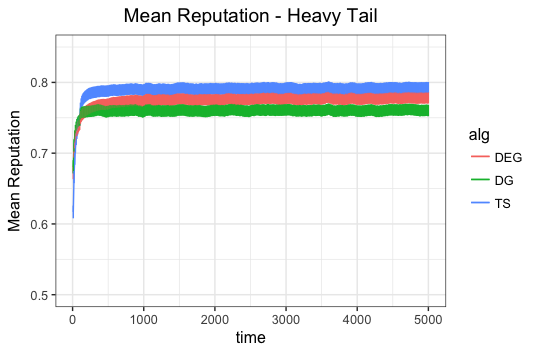
\includegraphics[scale=0.35]{appendix_figures/mean_ht_3_arms} \\
\end{center}

Finally, the relative reputation trajectory of \DEG vs. \DG:
\begin{center}
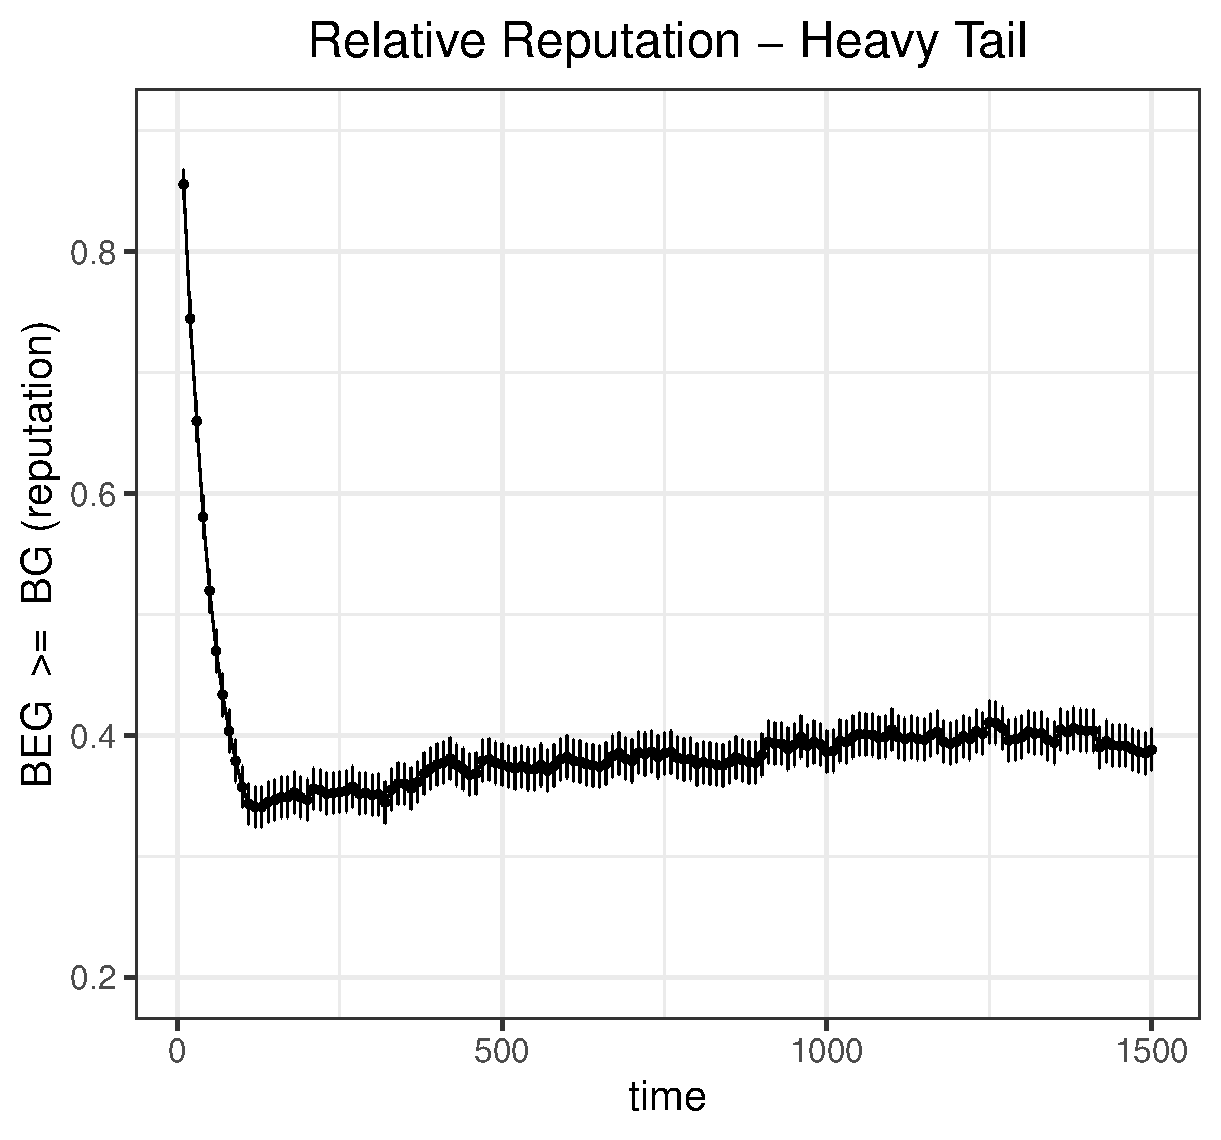
\includegraphics[scale=0.35]{appendix_figures/rel_rep_ht_3_arms}
\end{center}

%\end{appendices}


\end{document}
